\documentclass[12pt]{article}
\usepackage{listings}
\usepackage{graphicx}
\usepackage{xcolor}

\begin{document}
\title{ECEC 471 Lab 6}
\author{Nicholas Sica}
\date{November 23, 2020}
\maketitle

\section{Introduction}
\subsection{Overview}
This lab is meant to use the knowledge gained in the previous labs to build an edge-triggered flip-flop.
An edge-triggered flip-flop is a device that saves whatever state is at the input every rising edge of
the clock signal. It is a type of memory and is essential to sequential digital logic design.
Rise time and fall time are the time it takes for the ouput to rise from 20\% to 80\% of the total
voltage or fall from 80\% to 20\% of the total voltage. Propagation delay is the time it takes for
the output to appear after the input, usually measured by taking the difference of the 50\% marks
of the input and output. The propagation delay is measured using the rising edge of the clock as
the input. Two new concepts called setup and hold time were also introduced. The setup time is the
minimum time that is needed for the data to be stable before the rising edge of the clock. The hold
time is how long after the rising edge of the clock the data needs to be stable. Violation of these
times can cause a flip-flop to not be able to save the state correctly.
\section{Simulation and Analysis}
\subsection{Schematic Design}
Figure~\ref{fig:schem} shows the transistor-level schematic of the edge-triggered flip-flop.
It is made up of five 2-input nand gates and one 3-input nand. The width of all the devices is the
default symmetric version of that gate.
\begin{figure}[!htb]
  \centering
  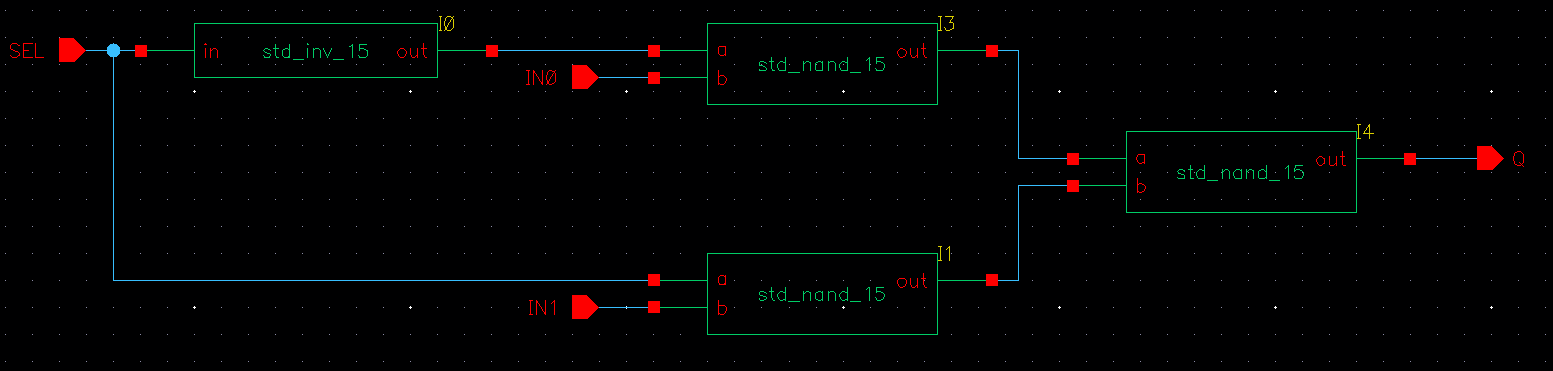
\includegraphics[width=5in]{figures/schem.png}
  \caption{Transistor-level Edge-Triggered Flip-Flop Schematic}\label{fig:schem}
\end{figure}
Figure~\ref{fig:sim} shows the simulation schematic with the source and load. 
Two different pulses are used, one acting as the clock and the other acting as the data.
All the pulses have an amplitude of 1.2V, a rise time of 10ps, and a fall time of 10ps.
While the clock has a pulse width of 240ps and a period of 500ps, the data has a pulse width of 45ps,
a delay of 494.5ps, and a period of 1ns.
A 5fF capacitor was tied to each output to get it closer to a realistic model where the output would have some capacitance.
\begin{figure}[!htb]
  \centering
  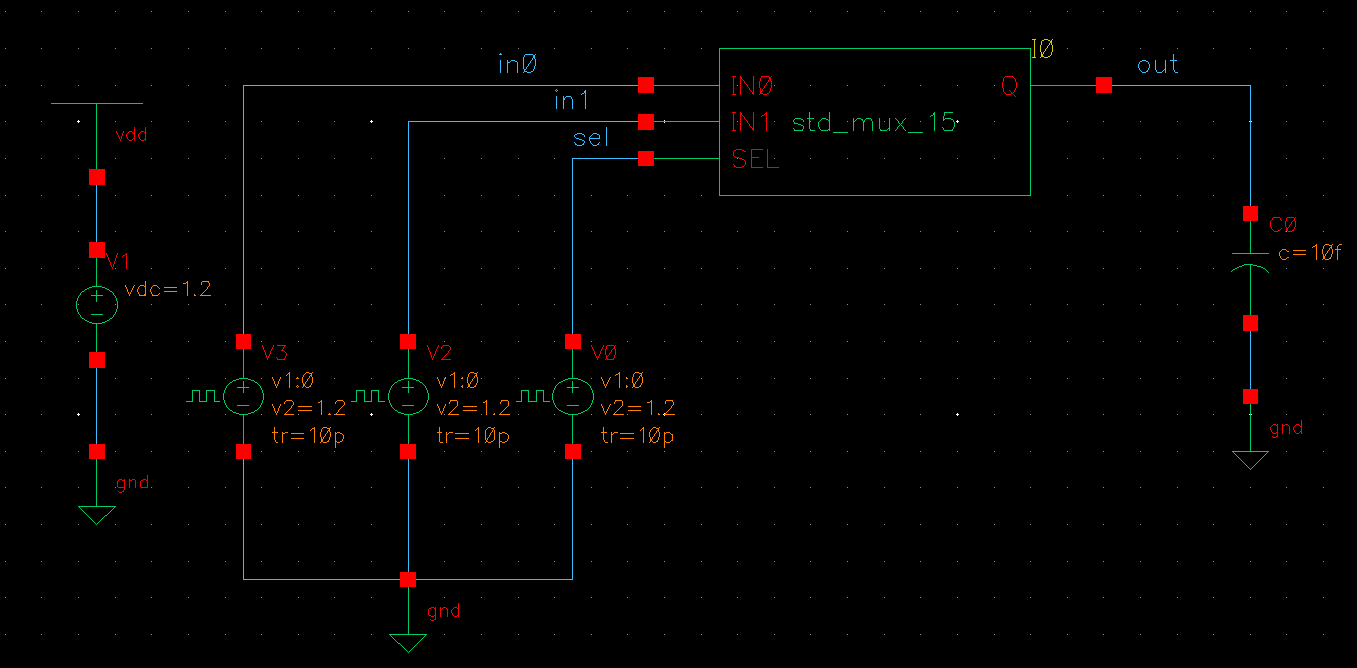
\includegraphics[width=5in]{figures/sim.png}
  \caption{Edge-Triggered Flip-Flop Simulation Schematic}\label{fig:sim}
\end{figure}
The transient analysis is shown in Figure~\ref{fig:transient}. Using the transient analysis graph a
rise time of 58.3657ps, a fall time of 35.6452ps, and a clock-to-q propagation delay of 80.4614ps were all
easily found. Setup and hold time were found by setting the delay and width of the data to a variable
and doing a parametric sweep to find the minimum time where the flip-flop would still work.
The setup and hold time were found to be 5.5ps and 49.5ps, respectively.
\begin{figure}[!htb]
  \centering
  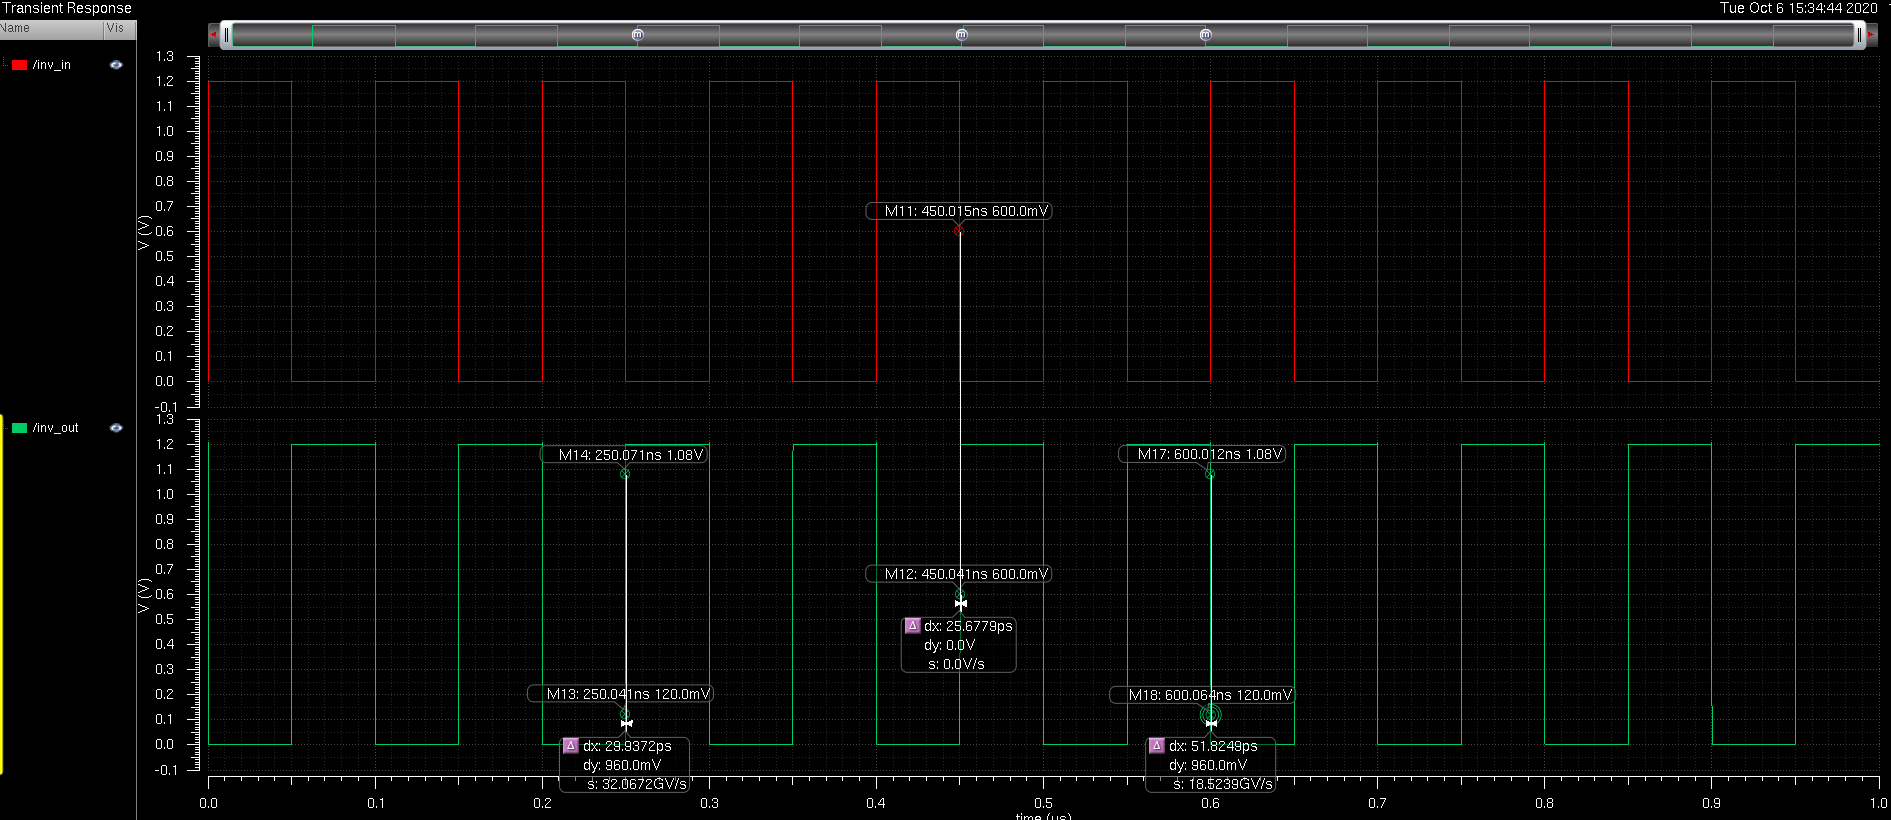
\includegraphics[width=5in]{figures/transient.png}
  \caption{Edge-Triggered Flip-Flop Transient Analysis}\label{fig:transient}
\end{figure}
\subsection{Layout Design}
After the edge-triggered flip-flop's schematic was finished, layout was done. The layout was done using
pitch matching and using the previous layouts that were created for the symmetric gates.
After the gates' layouts were place metal was placed between the designs and the pins were
placed. A second metal was also used to route parts that are supposed to be tied together, but are
on opposite sides of the design. The layout is shown in Figure~\ref{fig:layout}.
\begin{figure}[!htb]
  \centering
  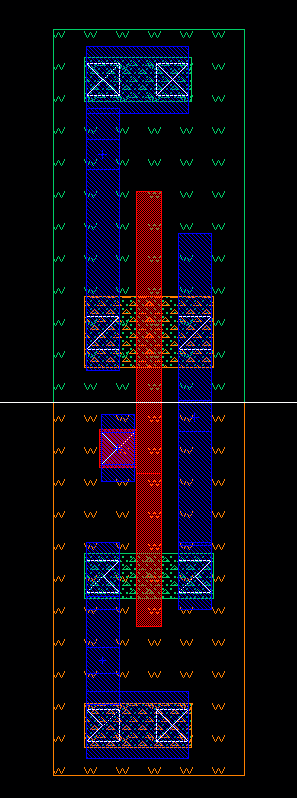
\includegraphics[width=5in]{figures/layout.png}
  \caption{Edge-Triggered Flip-Flop Layout}\label{fig:layout}
\end{figure}
Lastly, design rule checking(DRC) is used to make sure that no design rules are being violated and
everything is fixed very painstakingly. The results for the design rule checking are shown in
Figure~\ref{fig:drc}. After that layout versus schematic(LVS) was used to make sure the layout matches
the design modeled with the schematic and is shown in Figure~\ref{fig:lvs}.
\begin{figure}[!htb]
  \centering
  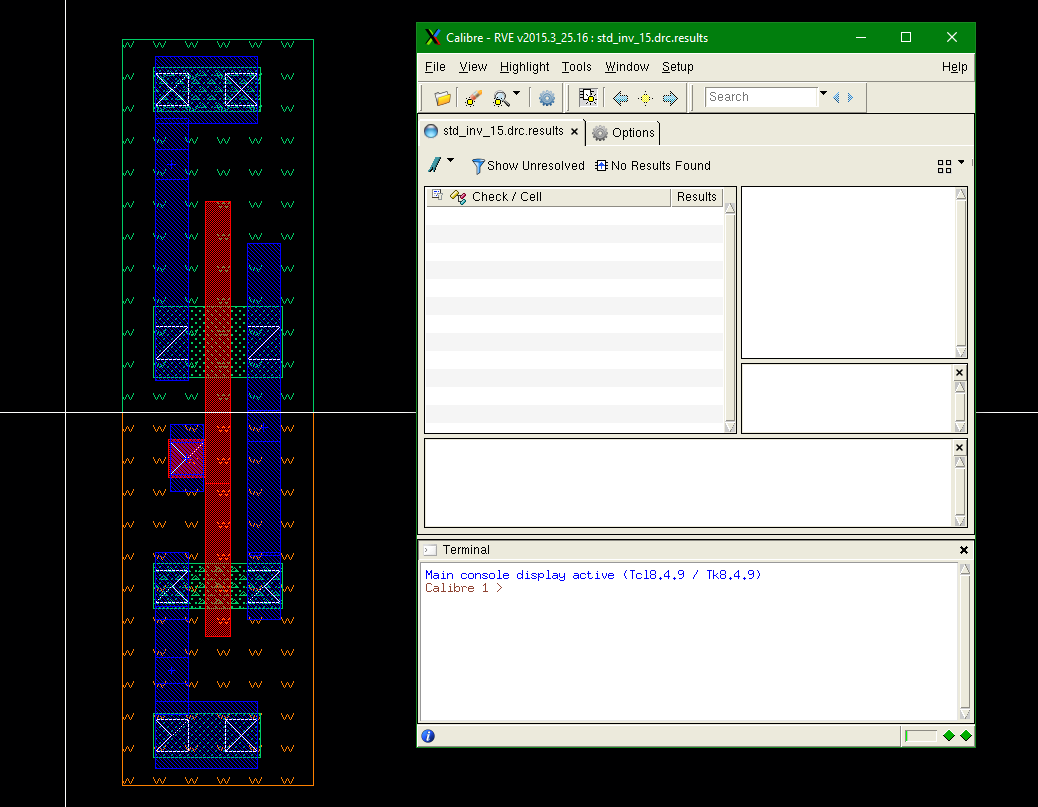
\includegraphics[width=3.5in]{figures/drc.png}
  \caption{DRC Results}\label{fig:drc}
\end{figure}
\begin{figure}[!htb]
  \centering
  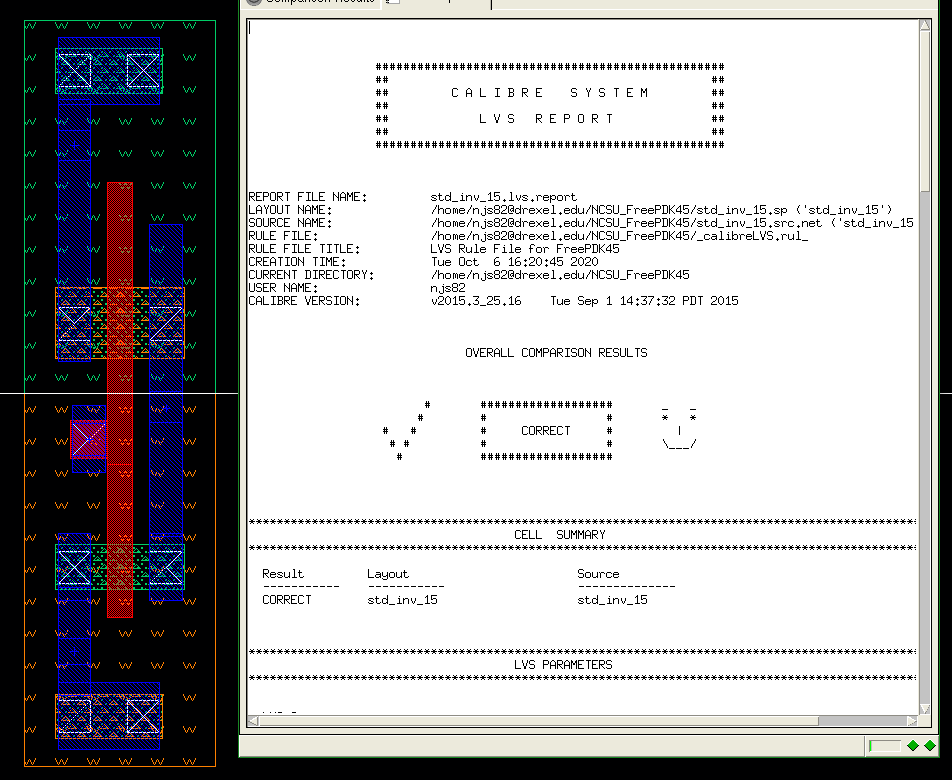
\includegraphics[width=3.5in]{figures/lvs.png}
  \caption{LVS Results}\label{fig:lvs}
\end{figure}
\clearpage
\section{Conclusion}
The lab was a great way to cement everything that was learned previously and get even further experience
creating a layout with previously designed gates. Pitch matching saves a lot of time in the long run and
allows heavy design reuse. It also helped in tracking down any issues as the designs of the gates have
been verified, so if there was anything wrong, it was easy to figure out that it was in the interconnection
of the separate gates. It also helped us through figuring out the minimum setup and hold time needed for
a specific piece of sequential logic.
\end{document}
%%% Local Variables:
%%% mode: latex
%%% TeX-master: t
%%% End:
